\documentclass[a4paper,10pt,landscape]{article}
\usepackage{multicol}
\usepackage{calc}
\usepackage{ifthen}
\usepackage[landscape]{geometry}
\usepackage{graphicx}
\usepackage{amsmath, amssymb, amsthm}
\usepackage{latexsym, marvosym}
\usepackage{pifont}
\usepackage{lscape}
\usepackage{dsfont}
\usepackage{graphicx}
\usepackage{array}
\usepackage{booktabs}
\usepackage[bottom]{footmisc}
\usepackage{tikz}
\usetikzlibrary{shapes}
\usepackage{pdfpages}
\usepackage{wrapfig}
\usepackage{enumitem}
\setlist[description]{leftmargin=0pt}
\usepackage{xfrac}
\usepackage[pdftex,
            pdfauthor={Janus Advincula},
            pdftitle={Probability -- The Science of Uncertainty and Data},
            pdfsubject={A cheatsheet pdf and reference guide made for MIT's 6.431x course.},
            pdfkeywords={probability} {statistics} {cheatsheet} {pdf} {cheat} {sheet} {formulas} {equations}
            ]{hyperref}
\usepackage[
            open,
            openlevel=2
            ]{bookmark}
\usepackage{relsize}
\usepackage{rotating}

 \newcommand\independent{\protect\mathpalette{\protect\independenT}{\perp}}
    \def\independenT#1#2{\mathrel{\setbox0\hbox{$#1#2$}%
    \copy0\kern-\wd0\mkern4mu\box0}} 
            
\newcommand{\noin}{\noindent}    
\newcommand{\logit}{\textrm{logit}} 
\newcommand{\var}{\textrm{Var}}
\newcommand{\cov}{\textrm{Cov}} 
\newcommand{\corr}{\textrm{Corr}} 
\newcommand{\N}{\mathcal{N}}
\newcommand{\Bern}{\textrm{Bern}}
\newcommand{\Bin}{\textrm{Bin}}
\newcommand{\Beta}{\textrm{Beta}}
\newcommand{\Gam}{\textrm{Gamma}}
\newcommand{\Expo}{\textrm{Expo}}
\newcommand{\Pois}{\textrm{Pois}}
\newcommand{\Unif}{\textrm{Unif}}
\newcommand{\Geom}{\textrm{Geom}}
\newcommand{\NBin}{\textrm{NBin}}
\newcommand{\Hypergeometric}{\textrm{HGeom}}
\newcommand{\HGeom}{\textrm{HGeom}}
\newcommand{\Mult}{\textrm{Mult}}

\geometry{top=.4in,left=.2in,right=.2in,bottom=.4in}

\pagestyle{empty}
\makeatletter
\renewcommand{\section}{\@startsection{section}{1}{0mm}%
                                {-1ex plus -.5ex minus -.2ex}%
                                {0.5ex plus .2ex}%x
                                {\normalfont\large\bfseries}}
\renewcommand{\subsection}{\@startsection{subsection}{2}{0mm}%
                                {-1explus -.5ex minus -.2ex}%
                                {0.5ex plus .2ex}%
                                {\normalfont\normalsize\bfseries}}
\renewcommand{\subsubsection}{\@startsection{subsubsection}{3}{0mm}%
                                {-1ex plus -.5ex minus -.2ex}%
                                {1ex plus .2ex}%
                                {\normalfont\small\bfseries}}
\makeatother

\setcounter{secnumdepth}{0}

\setlength{\parindent}{0pt}
\setlength{\parskip}{0pt plus 0.5ex}

% -----------------------------------------------------------------------

\usepackage{titlesec}

\titleformat{\section}
{\color{blue}\normalfont\large\bfseries}
{\color{blue}\thesection}{1em}{}
\titleformat{\subsection}
{\color{violet}\normalfont\normalsize\bfseries}
{\color{violet}\thesection}{1em}{}
% Comment out the above 5 lines for black and white

\begin{document}

\raggedright
\footnotesize
\begin{multicols*}{3}

% multicol parameters
% These lengths are set only within the two main columns
%\setlength{\columnseprule}{0.25pt}
\setlength{\premulticols}{1pt}
\setlength{\postmulticols}{1pt}
\setlength{\multicolsep}{1pt}
\setlength{\columnsep}{2pt}

%%%%%%%%%%%%%%%%%%%%%%%%%%%%%%%%%%%%
%%% TITLE
%%%%%%%%%%%%%%%%%%%%%%%%%%%%%%%%%%%%

\begin{center}
    {\color{blue} \Large{\textbf{6.431x Probability -- The Science of Uncertainty and Data}}} \\
   % {\Large{\textbf{Probability Cheatsheet}}} \\
    % comment out line with \color{blue} and uncomment above line for b&w
\end{center}

%%%%%%%%%%%%%%%%%%%%%%%%%%%%%%%%%%%%
%%% ATTRIBUTIONS
%%%%%%%%%%%%%%%%%%%%%%%%%%%%%%%%%%%%

\scriptsize

This is a cheat sheet for probability based on the online course given by Prof. John Tsitsiklis and Prof. Patrick Jaillet. Compiled by Janus B. Advincula.

\begin{center}
    Last Updated \today
\end{center}

% Cheatsheet format from
% http://www.stdout.org/$\sim$winston/latex/

%%%%%%%%%%%%%%%%%%%%%%%%%%%%%%%%%%%%
%%% BEGIN CHEATSHEET
%%%%%%%%%%%%%%%%%%%%%%%%%%%%%%%%%%%%


\section{Probability Models and Axioms}\smallskip \hrule height 1pt \smallskip

\subsection{Sample Space}
	
We begin by listing the possible outcomes, $\Omega$, of an experiment, i.e., the sample space. The list must be:
\begin{itemize}[label=\textcolor{red}{\textbullet}]
	\setlength\itemsep{-1pt}
	\item mutually exclusive,
	\item collectively exhaustive, and
	\item at the {\it right} granularity
\end{itemize}

\subsection{Probability Axioms}

An event, $A$, is a subset of the sample space. Probability is assigned to events with the following axioms:
\begin{itemize}[label=\textcolor{red}{\textbullet}]
	\setlength\itemsep{-1pt}
	\item Nonnegativity: $\mathds{P}(A)\geq0$
	\item Normalization: $\mathds{P}(\Omega)=1$
	\item (Finite) Additivity:
	
	If $A\cap B=\emptyset$, then $\mathds{P}(A\cap B)=\mathds{P}(A)+\mathds{P}(B)$.
\end{itemize}
\begin{description}
	\item[Consequences of the Axioms] ~
	\begin{itemize}[label=\textcolor{red}{\textbullet}]
		\setlength\itemsep{-1pt}
		\item $\mathds{P}(A)\leq1$
		\item $\mathds{P}(\emptyset)=0$
		\item $\mathds{P}(A)+\mathds{P}(A^\mathsf{c})=1$
		\item If $A\subset B$, then $\mathds{P}(A)\leq\mathds{P}(B)$
		\item \textbf{Union bound:} $\mathds{P}(A\cup B)\leq\mathds{P}(A)+\mathds{P}(B)$
	\end{itemize}
	\item[Countable Additivity Axiom] If $A_1, A_2, A_3, \dots$ is an infinite {\it sequence} of {\it disjoint} events, then
	\begin{gather*}
	\mathds{P}\left(A_1\cup A_2\cup \dots\right)=\mathds{P}\left(A_1\right)+\mathds{P}\left(A_2\right)+\dots\\
	\text{or}\quad\mathds{P}\left(\bigcup\limits_{i}A_i\right)=\sum_{i}\mathds{P}\left(A_i\right)
	\end{gather*}
	\item[Discrete Uniform Law] Assume that $\Omega$ is finite and consists of $n$ equally likely elements. Also, assume that $A\subset\Omega$ consists of $k$ elements. Then, $$\mathds{P}(A)=\frac{k}{n}.$$ 
\end{description}

\subsection{Mathematical Background}
\begin{description}
	\item[Sets] A set is a collection of distinct elements. $$x\in S\cup T\;\Leftrightarrow\;x\in S\;\textbf{or}\;x\in T$$ $$x\in S\cap T\;\Leftrightarrow\;x\in S\;\textbf{and}\;x\in T$$
	\item[De Morgan's Laws]
	\begin{align*} 
		\left(\bigcup\limits_{n}S_n\right)^\mathsf{\!c}&=\bigcap\limits_{n}S_n^\mathsf{\,c}\\
		\left(\bigcap\limits_{n}S_n\right)^\mathsf{\!c}&=\bigcup\limits_{n}S_n^\mathsf{\,c}
	\end{align*}
	\item[Geometric Series] $$S=\sum_{i=0}^{\infty}\alpha^i=1+\alpha+\alpha^2+\dots=\frac{1}{1-\alpha}$$
	\item[Bonferroni's Inequality] $$\mathds{P}(A_1\cap\dots\cap A_n)\geq\mathds{P}(A_1)+\dots+\mathds{P}(A_n)-(n-1)$$
\end{description}

\section{Conditioning and Independence} \smallskip \hrule height 1pt \smallskip

\subsection{Conditioning and Bayes' Rule}

\begin{description}
	\item[Conditional Probability] We denote the probability of $A$, given that $B$ occurred by $\mathds{P}(A|B)$ and this is defined as
	\begin{equation*}
		\mathds{P}(A|B)=\frac{\mathds{P}(A\cap B)}{\mathds{P}(B)}, \quad \mathds{P}(B)>0.
	\end{equation*}
	Conditional probabilities share properties of ordinary probabilities.
	\item[The multiplication rule] Given the definition of conditional probability, we have
	\begin{equation*}
	\setlength\abovedisplayskip{3pt}
		\mathds{P}(A\cap B)=\mathds{P}(B)\,\mathds{P}(A|B)=\mathds{P}(A)\,\mathds{P}(B|A).
	\end{equation*}
	In general, we have
	\begin{equation*}
		\setlength\abovedisplayskip{0pt}
		\mathds{P}\left(A_1\cap A_2\cap\dots\cap A_n\right)=\mathds{P}(A_1)\prod_{i=2}^{n}\mathds{P}\left(A_i|A_1\cap\dots\cap A_{i-1}\right)
		\setlength\belowdisplayskip{0pt}
	\end{equation*}
	\item[Total probability theorem] We partition the sample space into $A_1, A_2,A_3,\dots$ Then,
	\begin{align*}
		\mathds{P}(B) & = \mathds{P}(B\cap A_1) + \mathds{P}(B\cap A_2) + \mathds{P}(B\cap A_3) + \dots\\
		&=\mathds{P}(A_1)\mathds{P}(B|A_1)+\mathds{P}(A_2)\mathds{P}(B|A_2)+\mathds{P}(A_3)\mathds{P}(B|A_3)+\dots\\
		&=\sum_{i}\mathds{P}(A_i)\mathds{P}(B|A_i)
		\setlength\belowdisplayskip{0pt}
	\end{align*}
	\item[Bayes' Rule]
	\begin{equation*}
		\mathds{P}(A_i|B)=\frac{\mathds{P}(A_i)\mathds{P}(B|A_i)}{\sum\limits_{j}\mathds{P}(A_j)\mathds{P}(B|A_j)}
	\end{equation*}
\end{description}
\subsection{Independence}

    \begin{description}
        \item[Independence of Two Events] $A$ and $B$ are independent if knowing whether $A$ occurred gives no information about whether $B$ occurred. More formally, $A$ and $B$ (which have nonzero probability) are independent if and only if one of the following equivalent statements holds:
        \vspace{-1em}
           \begin{align*}
            \mathds{P}({A}\cap { B}) &= \mathds{P}({A})\mathds{P}({B}) \\
            \mathds{P}({ A}|{ B}) &= \mathds{P}({A})\\
            \mathds{P}(B|A) &= \mathds{P}(B)
           \end{align*}
        \vspace{-1em}
        \item[Independence of Event Complements] If $A$ and $B$ are independent, then $A$ and $B^\mathsf{\,c}$ are independent: $$\setlength\abovedisplayskip{2pt}\mathds{P}\left(A\cap B^\mathsf{\,c}\right)=\mathds{P}(A)\mathds{P}\left(B^\mathsf{\,c}\right)$$
        \vspace{-1em}
        \item[Conditional Independence]  ${A}$ and ${B}$ are conditionally independent given ${C}$ if $$\mathds{P}({A}\cap {B}|{C}) = \mathds{P}({A}|{C})\mathds{P}({B}|{C}).$$ Conditional independence does not imply independence, and independence does not imply conditional independence.
    \end{description}

\section{Counting}\smallskip \hrule height 1pt \smallskip

\subsection{Basic Counting Principle}
    For a selection that can be done in $r$ stages, with $n_i$ choices at each stage $i$, the number of possible selections is $$\setlength\abovedisplayskip{2pt}n_1n_2 \dots n_r.$$
\begin{description}
	\item[Permutations] The number of ways of ordering $n$ distinct elements is $$n!=1\cdot2\cdot3\cdots n.$$
	\item[Combinations] Given a set of $n$ elements, the number of ways of constructing an {\it ordered} sequence of $k$ {\it distinct} elements is
	$$\binom{n}{k}=\frac{n!}{k!(n-k)!}$$
	\item[Subsets] The number of subsets of $\{1,\dots,n\}$ is $$\sum_{k=0}^{n}\binom{n}{k}=\binom{n}{0}+\cdots+\binom{n}{n}=2^n.$$
	\item[Partitions] Given an $n$-element set and nonnegative integers $n_1,n_2,\dots,n_r$, whose sum is equal to $n$, the number of ways of partitioning the set into $r$ disjoint subsets, with the $i$\textsuperscript{th} subset containing exactly $n_i$ elements, is equal to $$\frac{n!}{n_1!n_2!\dots n_r!}.$$
\end{description}

\section{Discrete Random Variables}\smallskip \hrule height 1pt \smallskip
\subsection{Random Variables}
A random variable associates a value to every possible outcome. It can take discrete or continuous values.
\begin{description}
	
	\item[Probability Mass Function (PMF)] 
	Gives the probability that a \emph{discrete} random variable takes on the value $x$.
	\[ p_X(x) = \mathds{P}(X=x)=\mathds{P}(\{\omega\in\Omega:X(\omega)=x\}) \]
	The PMF satisfies
	\[p_X(x) \geq 0 \textrm{ and } \sum_x p_X(x) = 1. \]
	\item[Bernoulli random variable] A Bernoulli random variable $X$ with parameter $0\leq p\leq 1$, $X\sim$ Ber($p$), takes the following values:
	\[X=\left\{\begin{array}{ll}
	1,&\text{w.p. }p,\\
	0,&\text{w.p. }1-p.
	\end{array}\right.\]
	\item[Discrete uniform random variable] A discrete uniform random variable $X$ between $a$ and $b$, $X\sim\text{Uni}[a,b]$, takes any of the values $\{a,a+1,\dots,b\}$ with probability $\frac{1}{b-a+1}$.
	\item[Binomial random variable] A binomial random variable $X$ with parameter $n$ and $p\in[0,1]$, $X\sim\text{Bin}(n,p)$, takes values in the set $\{0,1,\dots,n\}$ and has PMF \[p_X(k)=\binom{n}{k}p^k(1-p)^{n-k},\quad\text{for }k=0,1,\dots,n.\]
	\item[Geometric random variable] A geometric random variable $X$ with parameter $p\in[0,1]$, $X\sim\text{Geo}(p)$, takes values in the set $\{1,2,\dots\}$ with probability \[p_X(k)=(1-p)^kp.\]
	\item[Expectation Value] The expectation value of a discrete random variable is defined as \[\mathds{E}\left[X\right]=\sum_xxp_X(x).\]
	\item[Expectation of a Bernoulli random variable] The expected value of a Bernoulli r.v. with parameter $p$ is \[\mathds{E}\left[X\right]=p.\]
	\item[Expectation of a Discrete Uniform random variable] The expected value of a discrete uniform r.v. is \[\mathds{E}\left[X\right]=\frac{b+a}{2}.\]
	\item[Properties of Expectations] ~
	\begin{itemize}[label=\textcolor{red}{\textbullet}]
		\item If $X\geq0$, then $\mathds{E}\left[X\right]\geq0.$
		\item If $a\leq X\leq b$, then $a\leq\mathds{E}\left[X\right]\leq b.$
		\item If $c$ is a constant, $\mathds{E}\left[c\right]=c.$
		\item Let $X$ be a r.v. and let $Y=g(X).$ Then, \[\mathds{E}\left[Y\right]=\mathds{E}\left[g(X)\right]=\sum_xg(x)p_X(x).\]
	\end{itemize}
	\item[Linearity of Expectation] \[\mathds{E}\left[aX+b\right]=a\mathds{E}\left[X\right]+b\]
	
\end{description}

\subsection{Variance and Standard Deviation}
\begin{description}
	\item[Definition of Variance] Variance is a measure of the spread of a PMF. For a random variable with mean $\mu=\mathds{E}[X]$, it is defined as \[\var(X) =\mathds{E}\left[\left(X-\mu\right)^2\right] = \mathds{E}\left[X^2\right]-\left(\mathds{E}\left[X\right]\right)^2.\]
	\item[Properties] \[\var(aX+b)=a^2\var(X)\]
	\item[Standard Deviation] 
	\[\sigma_X = \sqrt{\var(X)}\]
	\item[Variance of a Bernoulli random variable] \[\var(X)=p(1-p)\]
	\item[Variance of a Discrete Uniform random variable] \[\var(X)=\frac{1}{12}(b-a)(b-a+1)\]
\end{description}

\subsection{Conditional PMF and Expectation}
\begin{description}
	\item[Total Expectation Theorem] Given a random variable $X$ and events $A_1,\dots,A_n$, we have \[\mathds{E}\left[X\right]=\mathds{P}(A_1)\mathds{E}\left[X|A_1\right]+\dots+\mathds{P}(A_n)\mathds{E}\left[X|A_n\right].\]
\end{description}

\section{Continuous Random Variables}\smallskip \hrule height 1pt \smallskip

\subsection{Continuous Random Variables (CRVs)}
\begin{description}

\item[Definition] A random variable is continuous if it can be described by a PDF, $f_X(x)$, such that
\[\mathds{P}(a \leq X \leq a+\delta)\approx f_X(a)\cdot\delta.\]
\item[Expectation] Assuming that $\int_{-\infty}^{\infty}|x|f_X(x)dx<\infty$, the expected value of a random variable $X$ is $$\mathds{E}\left[X\right]=\int_{-\infty}^{\infty}xf_X(x)dx.$$
\item[Properties] ~
	\begin{itemize}[label=\textcolor{red}{\textbullet}]
		\setlength\itemsep{-1pt}
		\item If $X\geq0$, then $\mathds{E}[X]\geq0$.
		\item If $a\leq X\leq b$, then $a\leq\mathds{E}[X]\leq b$.
		\item  $$\mathds{E}\left[g(X)\right]=\int_{-\infty}^{\infty}g(x)f_X(x)dx$$
		\item $\mathds{E}[aX+b]=a\mathds{E}[X]+b$
	\end{itemize}
\item[What is the Probability Density Function (PDF)?] The PDF $f$ is the derivative of the CDF $F$.
\[ F'(x) = f(x) \]
A PDF is nonnegative and integrates to $1$. By the fundamental theorem of calculus, to get from PDF back to CDF we can integrate:
\begin{align*} 
    F(x) &=  \int_{-\infty}^x f(t)dt  
   \end{align*}
   \begin{minipage}{\linewidth}
            \centering
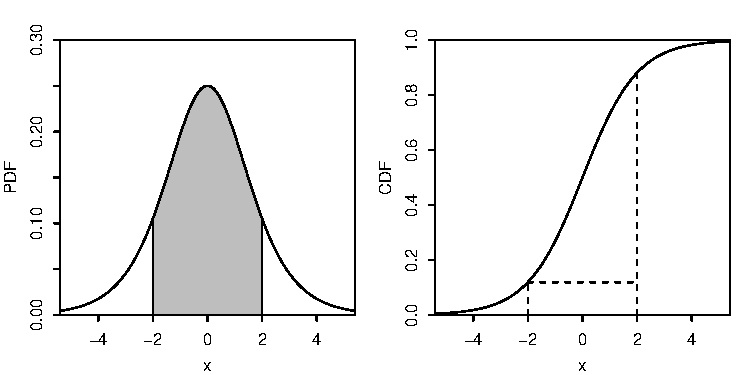
\includegraphics[width=2in]{figures/Logisticpdfcdf.pdf}
        \end{minipage}
   To find the probability that a CRV takes on a value in an interval, integrate the PDF over that interval.
      \begin{align*} 
    F(b) - F(a)  &=  \int^b_a f(x)dx
       \end{align*}
   
\end{description}


\section{Further Topics on Random Variables}\smallskip \hrule height 1pt \smallskip

\subsection{Covariance and Correlation}
\begin{description}
	\item [Covariance] is the analog of variance for two random variables.
	\[\cov(X, Y) = E\left((X - E(X))(Y - E(Y))\right) = E(XY) - E(X)E(Y)\]
	Note that 
	\[\cov(X, X) = E(X^2) - (E(X))^2 =  \var(X)\]
	\item [Correlation] is a standardized version of covariance that is always between $-1$ and $1$.
	\[\corr(X, Y) = \frac{\cov(X, Y)}{\sqrt{\var(X)\var(Y)}} \]
	\item [Covariance and Independence] If two random variables are independent, then they are uncorrelated. The converse is not necessarily true (e.g., consider $X \sim \N(0,1)$ and $Y=X^2$).
	\begin{align*}
	X \independent Y &\longrightarrow \cov(X, Y) = 0 \longrightarrow E(XY) = E(X)E(Y)
	\end{align*}
	%, except in the case of Multivariate Normal, where uncorrelated \emph{does} imply independence.
	\item [Covariance and Variance]  The variance of a sum can be found by
	\begin{align*}
	%\cov(X, X) &= \var(X) \\
	\var(X + Y) &= \var(X) + \var(Y) + 2\cov(X, Y) \\
	\var(X_1 + X_2 + \dots + X_n ) &= \sum_{i = 1}^{n}\var(X_i) + 2\sum_{i < j} \cov(X_i, X_j)
	\end{align*}
	If $X$ and $Y$ are independent then they have covariance $0$, so
	\[X \independent Y \Longrightarrow \var(X + Y) = \var(X) + \var(Y)\]
	If $X_1, X_2, \dots, X_n$ are identically distributed and have the same covariance relationships (often by \textbf{symmetry}), then 
	\[\var(X_1 + X_2 + \dots + X_n ) = n\var(X_1) + 2{n \choose 2}\cov(X_1, X_2)\]
	\item [Covariance Properties]  For random variables $W, X, Y, Z$ and constants $a, b$:
	\begin{align*}
	\cov(X, Y) &= \cov(Y, X) \\
	\cov(X + a, Y + b) &= \cov(X, Y) \\
	\cov(aX, bY) &= ab\cov(X, Y) \\
	\cov(W + X, Y + Z) &= \cov(W, Y) + \cov(W, Z) + \cov(X, Y)\\
	&\quad + \cov(X, Z)
	\end{align*}
	\item [Correlation is location-invariant and scale-invariant] For any constants $a,b,c,d$ with $a$ and $c$ nonzero,
	\begin{align*}
	\corr(aX + b, cY + d) &= \corr(X, Y) 
	\end{align*}
\end{description}

\subsection{A Deeper View of Conditioning}
\begin{description}
	\item[Conditional Expectation as a Random Variable] ~
	\[E\left[X|Y\right]=g(Y)\]
	\item[Law of Iterated Expectations] ~
	\[E\left[E\left[X|Y\right]\right]=E\left[X\right]\]
	\item[Law of Total Variance] ~
	\[\var(X)=E\left[\var\left(X|Y\right)\right]+\var\left(E\left[X|Y\right]\right)\]
	\item[Sum of a Random Number of Independent RVs] Let $Y=X_1+\dots+X_N$ where $N$ is a random variable. Then,
	\begin{align*}
		\var(Y)&=E\left[\var(Y|N)\right]+\var\left(E\left[Y|N\right]\right)\\
		&=E[N]\,\var(X)+\left(E[X]\right)^2\var(N)
	\end{align*}
\end{description}
\section{Bayesian Inference}\smallskip \hrule height 1pt \smallskip

Consider an unknown random variable $\Theta$ with a prior distribution $p_\Theta(\theta)$ or $f_\Theta(\theta)$. We make an observation $X$ modeled as a random variable with distribution $p_{X|\Theta}(x|\theta)$ or $f_{X|\Theta}(x|\theta)$. Using the appropriate version of the Bayes' rule, we can construct the appropriate posterior distribution $p_{\Theta|X}(\theta|x)$ or $f_{\Theta|X}(\theta|x).$

\subsection{Point Estimates}

\begin{description}
	\item[Maximum a posteriori probability (MAP)]  The MAP estimate, $\hat{\theta}$, is the value at which the posterior distribution is maximum: $$p_{\Theta|X}(\theta^*|x)=\max\limits_{\theta}p_{\Theta|X}(\theta|x)$$ $$f_{\Theta|X}(\theta^*|x)=\max\limits_{\theta}f_{\Theta|X}(\theta|x).$$
	\item[Least Mean Squares (LMS)] The LMS estimate is the conditional expectation of the posterior distribution: $$\hat{\theta}=\mathds{E}\left[\Theta|X=x\right].$$
\end{description}

\begin{description}
	\item[Discrete $\Theta$, Discrete $X$] ~
	
	$$p_{\Theta|X}(\theta|x)=\frac{p_\Theta(\theta)p_{X|\Theta}(x|\theta)}{p_X(x)}$$
	$$p_X(x)=\sum_{\theta'}p_\Theta(\theta')p_{X|\Theta}(x|\theta')$$
	
	\item[Discrete $\Theta$, Continuous $X$] ~
	
	$$p_{\Theta|X}(\theta|x)=\frac{p_\Theta(\theta)f_{X|\Theta}(x|\theta)}{f_X(x)}$$
	$$f_X(x)=\sum_{\theta'}p_\Theta(\theta')f_{X|\Theta}(x|\theta')$$
	
	\item[Continuous $\Theta$, Continuous $X$] ~
	
	$$f_{\Theta|X}(\theta|x)=\frac{f_\Theta(\theta)f_{X|\Theta}(x|\theta)}{f_X(x)}$$
	$$f_X(x)=\int f_\Theta(\theta')f_{X|\Theta}(x|\theta')d\theta'$$
	
	\item[Continuous $\Theta$, Discrete $X$] ~
	
	$$f_{\Theta|X}(\theta|x)=\frac{f_\Theta(\theta)p_{X|\Theta}(x|\theta)}{p_X(x)}$$
	$$p_X(x)=\int f_\Theta(\theta')p_{X|\Theta}(x|\theta')d\theta'$$
	
\end{description}

\subsection{Linear Least Mean Squares (LLMS) Estimation}
In some cases, the conditional expectation $\mathds{E}[\Theta|X]$ may be hard to compute or implement. In that case, we can restrict our attention to estimators of the form $\hat{\Theta}=aX+b.$ Then,
\begin{align*}
	\hat{\Theta}_\text{LLMS}&=\mathds{E}[\Theta]+\frac{\cov(\Theta,X)}{\var(X)}\left(X-\mathds{E}[X]\right)\\
	&=\mathds{E}[\Theta]+\rho\frac{\sigma_\Theta}{\sigma_X}\left(X-\mathds{E}[X]\right)
\end{align*}


\section{Limit Theorems and Classical Statistics}\smallskip \hrule height 1pt \smallskip
\subsection{Markov Inequality}
If $X\geq0$ and $a>0$, then $$\mathds{P}(X\ge a)\leq\frac{\mathds{E}\left[X\right]}{a}.$$
\subsection{Chebyshev Inequality}
If the variance is small, then $X$ is unlikely to be too far from the mean. $$\mathds{P}\left(\left|X-\mu\right|\ge c\right)\leq\frac{\sigma^2}{c^2}$$

\subsection{The Weak Law of Large Numbers (WLLN)}
Let $X_1, X_2, X_3, \dots$ be i.i.d.~with mean $\mu$ and variance $\sigma^2$. The \textbf{sample mean} is $$M_n = \frac{X_1 + \dots + X_n}{n}.$$ The \textbf{Weak Law of Large Numbers} states that: $$\text{for }\epsilon>0, \mathds{P}\left(\left|M_n-\mu\right|\ge\epsilon\right)\rightarrow0, \text{ as } n\rightarrow\infty.$$

\subsection{Transformations}
\begin{description}
    \label{one variable transformations}
    \item[One Variable Transformations] Let's say that we have a random variable $X$ with PDF $f_X(x)$, but we are also interested in some function of $X$. We call this function $Y = g(X)$. Also let $y=g(x)$. If $g$ is differentiable and strictly increasing (or strictly decreasing), then the PDF of $Y$ is
    \[f_Y(y) = f_X(x)\left|\frac{dx}{dy}\right| =  f_X(g^{-1}(y))\left|\frac{d}{dy}g^{-1}(y)\right|\]
    The derivative of the inverse transformation is called the \textbf{Jacobian}.


     \item[Two Variable Transformations] Similarly, let's say we know the joint PDF of $U$ and $V$ but are also interested in the random vector $(X, Y)$ defined by $(X, Y) = g(U, V)$. Let 
       $$  \frac{\partial (u,v)}{\partial (x,y)}  = \begin{pmatrix} 
              \frac{\partial u}{\partial x} &  \frac{\partial u}{\partial y} \\
           \frac{\partial v}{\partial x} & \frac{\partial v}{\partial y}   \\
        \end{pmatrix}$$
     be the \textbf{Jacobian matrix}. If the entries in this matrix exist and are continuous, and the determinant of the matrix is never $0$, then
     \[f_{X,Y}(x, y) = f_{U,V}(u,v) \left|\left|   \frac{\partial (u,v)}{\partial (x,y)}\right| \right| \]
   The inner bars tells us to take the matrix's determinant, and the outer bars tell us to take the absolute value.  In a $2 \times 2$ matrix, 
     \[ \left| \left|
     \begin{array}{ccc}
         a & b \\
         c & d
     \end{array}
     \right| \right| = |ad - bc|\]

\end{description}

\label{convolutions}
\subsection{Convolutions}
\begin{description}
    \item[Convolution Integral] If you want to find the PDF of the sum of two independent CRVs $X$ and $Y$, you can do the following integral:
        \[f_{X+Y}(t)=\int_{-\infty}^\infty f_X(x)f_Y(t-x)dx\]
    \item[Example] Let $X,Y \sim \N(0,1)$ be i.i.d. Then for each fixed $t$,\[f_{X+Y}(t)=\int_{-\infty}^\infty \frac{1}{\sqrt{2\pi}}e^{-x^2/2} \frac{1}{\sqrt{2\pi}}e^{-(t-x)^2/2} dx\]
By completing the square and using the fact that a Normal PDF integrates to $1$, this works out to $f_{X+Y}(t)$ being the $\N(0,2)$ PDF.
\end{description}

\section{Bernoulli and Poisson Processes}\smallskip \hrule height 2pt \smallskip

\begin{description}
\item[Definition] We have a \textbf{Poisson process} of rate $\lambda$ arrivals per unit time if the following conditions hold:
\begin{enumerate}
    \item The number of arrivals in a time interval of length $t$ is $\Pois(\lambda t)$.
    \item Numbers of arrivals in disjoint time intervals are independent.
\end{enumerate}
For example, the numbers of arrivals in the time intervals $[0,5]$, $(5,12),$ and $[13,23)$ are independent with $\Pois(5\lambda), \Pois(7\lambda), \Pois(10\lambda)$ distributions, respectively.
\begin{minipage}{\linewidth}
            \centering
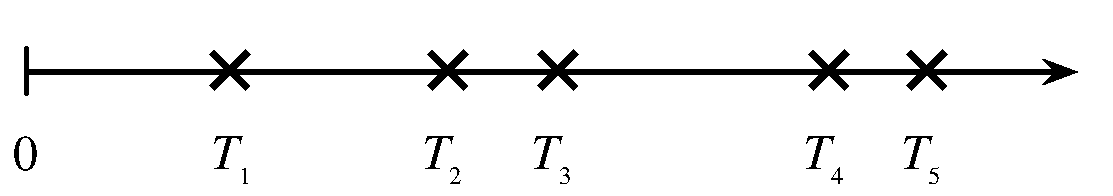
\includegraphics[width=2in]{figures/pp.pdf}
        \end{minipage}
       
\item[Count-Time Duality]  Consider a Poisson process of emails arriving in an inbox at rate $\lambda$ emails per hour. Let $T_n$ be the time of arrival of the $n$th email (relative to some starting time $0$) and $N_t$ be the number of emails that arrive in $[0,t]$. Let's find the distribution of $T_1$. The event $T_1 > t$, the event that you have to wait more than $t$ hours to get the first email, is the same as the event $N_t = 0$, which is the event that there are no emails in the first $t$ hours. So
\[P(T_1 > t) = P(N_t = 0) = e^{-\lambda t} \longrightarrow P(T_1 \leq t) = 1 - e^{-\lambda t}\]
Thus we have $T_1 \sim \Expo(\lambda)$. By the memoryless property and similar reasoning, the interarrival times between emails are i.i.d.~$\Expo(\lambda)$, i.e., the differences $T_n - T_{n-1}$ are i.i.d.~$\Expo(\lambda)$.
\end{description}

\section{Order Statistics}\smallskip \hrule height 2pt \smallskip
\begin{description}
    \item[Definition] Let's say you have $n$ i.i.d.~r.v.s $X_1, X_2,\dots, X_n$. If you arrange them from smallest to largest, the $i$th element in that list is the $i$th order statistic, denoted $X_{(i)}$. So $X_{(1)}$ is the smallest in the list and $X_{(n)}$ is the largest in the list. \smallskip
    
     Note that the order statistics are \emph{dependent}, e.g., learning $X_{(4)} = 42$ gives us the information that $X_{(1)},X_{(2)},X_{(3)}$ are $\leq 42$ and $X_{(5)},X_{(6)},\dots,X_{(n)}$ are $\geq 42$.
    \item[Distribution]  Taking $n$ i.i.d. random variables $X_1, X_2, \dots, X_n$ with CDF $F(x)$ and PDF $f(x)$, the CDF and PDF of $X_{(i)}$ are:
        \[F_{X_{(i)}}(x) = P (X_{(i)} \leq x) = \sum_{k=i}^n {n \choose k} F(x)^k(1 - F(x))^{n - k}\]
    \[f_{X_{(i)}}(x) = n{n - 1 \choose i - 1}F(x)^{i-1}(1 - F(x))^{n-i}f(x)\]
%    \item[Universality of the Uniform] Let $X_1,X_2,\dots,X_n$ be i.i.d.~CRVs with CDF $F$, and let $U_j=F(X_j)$. By UoU, $U_1,U_2,\dots,U_n$ are i.i.d.~$\Unif(0,1)$. Since $F$ is increasing, $F(X_{(1)}) \leq F(X_{(2)}) \leq \dots \leq F(X_{(n)})$, so $U_{(j)} = F(X_{(j)})$.
    \item[Uniform Order Statistics]  The $j$th order statistic of i.i.d.~$U_1,\dots,U_n \sim \Unif(0,1)$ is $U_{(j)} \sim \Beta(j, n - j + 1)$.
\end{description}



\section{MVN, LLN, CLT}\smallskip \hrule height 2pt \smallskip



\subsection{Central Limit Theorem (CLT)}
\subsubsection{Approximation using CLT}
We use $\dot{\,\sim\,}$ to denote \emph{is approximately distributed}. We can use the \textbf{Central Limit Theorem} to approximate the distribution of a random variable $Y=X_1+X_2+\dots+X_n$ that is a sum of $n$ i.i.d. random variables $X_i$. Let  $E(Y) = \mu_Y$ and $\var(Y) = \sigma^2_Y$. The CLT says
\[Y \dot{\,\sim\,} \N(\mu_Y, \sigma^2_Y)\]
If the $X_i$ are i.i.d.~with mean $\mu_X$ and variance $\sigma^2_X$, then $\mu_Y = n \mu_X$ and $\sigma^2_Y = n \sigma^2_X$. For the sample mean $\bar{X}_n$, the CLT says
\[ \bar{X}_n = \frac{1}{n}(X_1 + X_2 + \dots + X_n) \dot{\,\sim\,} \N(\mu_X, \sigma^2_X/n) \]


\subsubsection{Asymptotic Distributions using CLT}

We use $\xrightarrow{D}$ to denote \emph{converges in distribution to} as $n  \to \infty$. The CLT says that if we standardize the sum $X_1 + \dots + X_n$  then the distribution of the sum converges to $\N(0,1)$ as $n \to \infty$:
\[\frac{1}{\sigma\sqrt{n}} (X_1 + \dots + X_n - n\mu_X) \xrightarrow{D} \N(0, 1)\]
In other words, the CDF of the left-hand side goes to the standard Normal CDF, $\Phi$. In terms of the sample mean, the CLT says
\[ \frac{\sqrt{n} (\bar{X}_n - \mu_X)}{\sigma_X} \xrightarrow{D} \N(0, 1)\]

\section{Markov Chains}\smallskip \hrule height 2pt \smallskip

\subsection{Definition}
\begin{minipage}{\linewidth}
            \centering
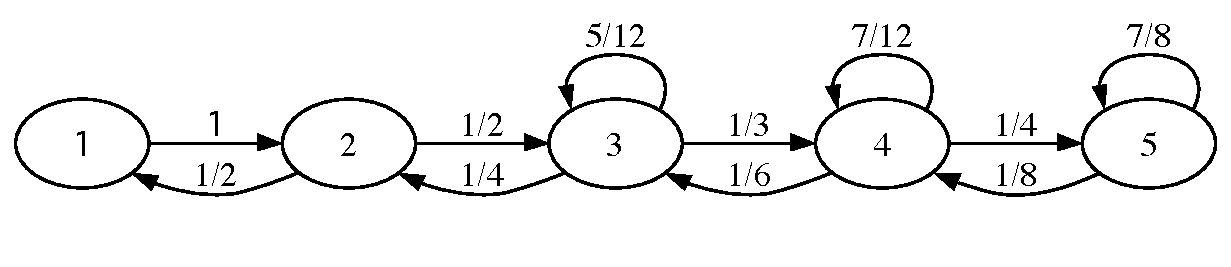
\includegraphics[width=2.3in]{figures/chainA.pdf}
        \end{minipage}
A Markov chain is a random walk in a \textbf{state space}, which we will assume is finite, say $\{1, 2, \dots, M\}$. We let $X_t$ denote which element of the state space the walk is visiting at time $t$. The Markov chain is the sequence of random variables tracking where the walk is at all points in time, $X_0, X_1, X_2, \dots$. By definition, a Markov chain must satisfy the \textbf{Markov property}, which says that if you want to predict where the chain will be at a future time, if we know the present state then the entire past history is irrelevant.  \emph{Given the present, the past and future are conditionally independent}. In symbols,
\[P(X_{n+1} = j | X_0 = i_0, X_1 = i_1, \dots, X_n = i) = P(X_{n+1} = j | X_n = i)\]
\subsection{State Properties}
A state is either recurrent or transient.
\begin{itemize}
\item If you start at a \textbf{recurrent state}, then you will always return back to that state at some point in the future.  \textmusicalnote \emph{You can check-out any time you like, but you can never leave.}  \textmusicalnote
\item Otherwise you are at a \textbf{transient state}. There is some positive probability that once you leave you will never return. \textmusicalnote \emph{You don't have to go home, but you can't stay here.} \textmusicalnote
\end{itemize}
A state is either periodic or aperiodic.
\begin{itemize}
\item If you start at a \textbf{periodic state} of period $k$, then the GCD of  the possible numbers of steps it would take to return back is  $k>1$.
\item Otherwise you are at an \textbf{aperiodic state}. The GCD of  the possible numbers of steps it would take to return back is 1.
\end{itemize}


\subsection{Transition Matrix}
Let the state space be $\{1,2,\dots,M\}$. The transition matrix $Q$ is the $M \times M$ matrix where element $q_{ij}$ is the probability that the chain goes from state $i$ to state $j$ in one step:
\[q_{ij} = P(X_{n+1} = j | X_n = i)\]

To find the probability that the chain goes from state $i$ to state $j$ in exactly $m$ steps, take the $(i, j)$ element of $Q^m$.
\[q^{(m)}_{ij} = P(X_{n+m} = j | X_n = i)\]
If $X_0$ is distributed according to the row vector PMF $\vec{p}$, i.e., $p_j = P(X_0 = j)$, then the PMF of $X_n$ is $\vec{p}Q^n$.



\subsection{Chain Properties}
A chain is \textbf{irreducible} if you can get from anywhere to anywhere. If a chain (on a finite state space) is irreducible, then all of its states are recurrent. A chain is \textbf{periodic} if any of its states are periodic, and is \textbf{aperiodic} if none of its states are periodic. In an irreducible chain, all states have the same period. \medskip

A chain is \textbf{reversible} with respect to $\vec{s}$ if $s_iq_{ij} = s_jq_{ji}$ for all $i, j$.  Examples of reversible chains include any chain with $q_{ij} = q_{ji}$, with $\vec{s} = (\frac{1}{M}, \frac{1}{M}, \dots, \frac{1}{M})$, and random walk on an undirected network.

\subsection{Stationary Distribution}

Let us say that the vector $\vec{s} = (s_1, s_2, \dots, s_M)$ be a PMF  (written as a row vector). We will call $\vec{s}$ the \textbf{stationary distribution} for the chain if $\vec{s}Q = \vec{s}$. As a consequence, if $X_t$ has the stationary distribution, then all future $X_{t+1}, X_{t + 2}, \dots$ also have the stationary distribution. \\

\smallskip

For irreducible, aperiodic chains, the stationary distribution exists, is unique, and $s_i$ is the long-run probability of a chain being at state $i$. The expected number of steps to return to $i$ starting from $i$ is $1/s_i$.

\smallskip

 To find the stationary distribution, you can solve the matrix equation $(Q' - I){\vec{s}\,}'= 0$. The stationary distribution is uniform if the columns of $Q$ sum to 1.

\smallskip

\textbf{Reversibility Condition Implies Stationarity}  If you have a PMF $\vec{s}$ and a Markov chain with transition matrix $Q$, then $s_iq_{ij} = s_jq_{ji}$ for all states $i, j$ implies that $\vec{s}$ is stationary.

\subsection{Random Walk on an Undirected Network}
 \begin{minipage}{\linewidth}
            \centering
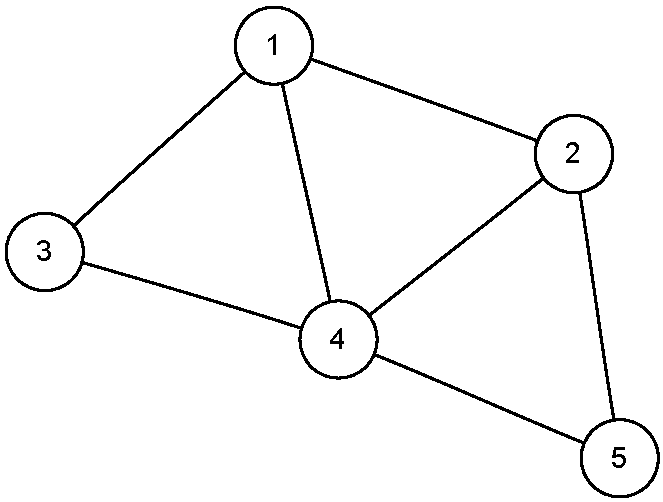
\includegraphics[width=1.6in]{figures/network1.pdf}
        \end{minipage}
\medskip

If you have a collection of \textbf{nodes}, pairs of which can be connected by undirected \textbf{edges}, and a Markov chain is run by going from the current node to a uniformly random node that is connected to it by an edge, then  this is a random walk on an undirected network. The stationary distribution of this chain is proportional to the \textbf{degree sequence} (this is the sequence of degrees, where the degree of a node is how many edges are attached to it). For example, the stationary distribution of random walk on the network shown above is proportional to $(3,3,2,4,2)$, so it's $(\frac{3}{14}, \frac{3}{14}, \frac{2}{14}, \frac{4}{14}, \frac{2}{14})$. 

\section{Continuous Distributions}\smallskip \hrule height 2pt \smallskip

\subsection{Uniform Distribution} Let us say that $U$ is distributed $\Unif(a, b)$. We know the following:
\begin{description}
    \item[Properties of the Uniform] For a Uniform distribution, the probability of a draw from any interval within the support is proportional to the length of the interval. See  \emph{Universality of Uniform} and \emph{Order Statistics} for other properties.
     \item[Example] William throws darts really badly, so his darts are uniform over the whole room because they're equally likely to appear anywhere. William's darts have a Uniform distribution on the surface of the room. The Uniform is the only distribution where the probability of hitting in any specific region is proportional to the length/area/volume of that region, and where the density of occurrence in any one specific spot is constant throughout the whole support.
%     \item[PDF and CDF (top is Unif(0, 1), bottom is Unif(a, b))]  
% \begin{eqnarray*}
% %\Unif(0, 1)
%   %\hspace{.7 in}
%    f(x) = \left\{
%      \begin{array}{lr}
%        1 & x \in [0, 1] \\
%        0 &  x \notin [0, 1]
%      \end{array}
%    \right.
%    %\hspace{.95 in}
%    F(x) = \left\{
%      \begin{array}{lr}
%        0 & x < 0 \\
%        x & x \in [0, 1] \\
%        1 &  x > 1
%      \end{array}
%    \right.\\
% %\Unif(a, b)
%   %\hspace{.65 in}
%    f(x) = \left\{
%      \begin{array}{lr}
%        \frac{1}{b-a} & x \in [a, b] \\
%        0 &  x \notin [a, b]
%      \end{array}
%    \right.
%    %\hspace{.75 in}
%    F(x) = \left\{
%      \begin{array}{lr}
%        0 & x < a \\
%        \frac{x-a}{b-a} & x \in [a, b] \\
%        1 &  x > b
%      \end{array}
%    \right. 
% \end{eqnarray*}


    
\end{description}

\subsection{Normal Distribution} Let us say that $X$ is distributed $\N(\mu, \sigma^2)$. We know the following:
\begin{description}
    \item[Central Limit Theorem] The Normal distribution is ubiquitous because of the Central Limit Theorem, which states that the sample mean of i.i.d.~r.v.s will approach a Normal distribution as the sample size grows, regardless of the initial distribution.
    \item[Location-Scale Transformation] Every time we shift a Normal r.v.~(by adding a constant) or rescale a Normal (by multiplying by a constant), we change it to another Normal r.v. For any Normal $X \sim \N(\mu, \sigma^2)$, we can transform it to the standard $\N(0, 1)$ by the following transformation:
    \[Z= \frac{X - \mu}{\sigma} \sim \N(0, 1) \]
%    \item[Example] Heights are normal. Measurement error is normal. By the central limit theorem, the sampling average from a population is also normal.
    \item[Standard Normal] The Standard Normal, $Z \sim \N(0, 1)$, has mean $0$ and variance $1$. Its CDF is denoted by $\Phi$.
\end{description}

\subsection{Exponential Distribution}

Let us say that $X$ is distributed $\Expo(\lambda)$. We know the following:
\begin{description}
    \item[Story] You're sitting on an open meadow right before the break of dawn, wishing that airplanes in the night sky were shooting stars, because you could really use a wish right now. You know that shooting stars come on average every 15 minutes, but a shooting star is  not ``due" to come just because you've waited so long. Your waiting time is memoryless;  the additional time until the next shooting star comes does not depend on how long you've waited already.
    
    \item[Example] The waiting time until the next shooting star is distributed $\Expo(4)$ hours. Here $\lambda=4$ is the \textbf{rate parameter}, since shooting stars arrive at a rate of $1$ per $1/4$ hour on average. The expected time until the next shooting star is $1/\lambda = 1/4$ hour.
    
    \item[Expos as a rescaled Expo(1)]
        \[Y \sim \Expo(\lambda) \rightarrow X = \lambda Y \sim \Expo(1)\]
     
%     \item[PDF and CDF] The PDF and CDF of a Exponential is:
% \[f(x) = \lambda e^{-\lambda x}, x \in [0, \infty)\]
% \[F(x) = P(X \leq x) = 1 - e^{-\lambda x}, x \in [0, \infty)\]
    
    \item[Memorylessness] The Exponential Distribution is the only continuous memoryless distribution. The memoryless property says that for $X \sim \Expo(\lambda)$ and any positive numbers $s$ and $t$,
    \[P(X > s + t | X > s) = P(X > t)\]
Equivalently,
    \[X - a | (X > a) \sim \Expo(\lambda)\]
    For example, a product with an $\Expo(\lambda)$ lifetime is always ``as good as new" (it doesn't experience wear and tear). Given that the product has survived $a$ years, the additional time that it will last is still $\Expo(\lambda)$. 

%    Example - If waiting for the bus is distributed exponentially with $\lambda = 6$, no matter how long you've waited so far, the expected additional waiting time until the bus arrives is always $\frac{1}{6}$, or 10 minutes. The distribution of time from now to the arrival is always the same, no matter how long you've waited.

    \item[Min of Expos] If we have independent $X_i \sim \Expo(\lambda_i)$, then $\min(X_1, \dots, X_k) \sim \Expo(\lambda_1 + \lambda_2 + \dots + \lambda_k)$. 
    \item[Max of Expos] If we have i.i.d.~$X_i \sim \Expo(\lambda)$, then $\max(X_1, \dots, X_k)$ has the same distribution as $Y_1+Y_2+\dots+Y_k$, where $Y_j \sim \Expo(j\lambda)$ and the $Y_j$ are independent.     
\end{description}

\subsection{Gamma Distribution}
\begin{minipage}{\linewidth}
            \centering
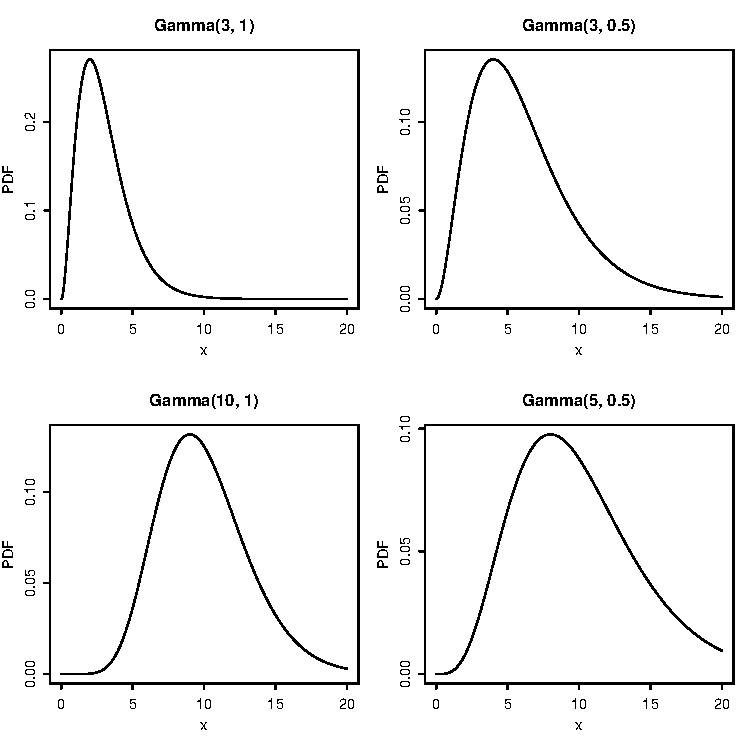
\includegraphics[width=1.9in]{figures/gammapdfs.pdf}
        \end{minipage}
\medskip
Let us say that $X$ is distributed $\Gam(a, \lambda)$. We know the following:
\begin{description}
    \item[Story] You sit waiting for shooting stars, where the waiting time for a star is distributed $\Expo(\lambda)$. You want to see $n$ shooting stars before you go home. The total waiting time for the $n$th shooting star is $\Gam(n,\lambda)$.
    \item[Example]  You are at a bank, and there are 3 people ahead of you. The serving time for each person is Exponential with mean $2$ minutes. Only one person at a time can be served. The distribution of your waiting time until it's your turn to be served is $\Gam(3, \frac{1}{2})$.
%     \item[PDF] The PDF of a Gamma is:
% \begin{eqnarray*}
% f(x) = \frac{1}{\Gamma(a)}(\lambda x)^ae^{-\lambda x}\frac{1}{x},
% \hspace{.1 in}
% x \in [0, \infty)
% \end{eqnarray*}
    % \item[Properties and Representations]

\end{description}

\subsection{Beta Distribution}
\begin{minipage}{\linewidth}
            \centering
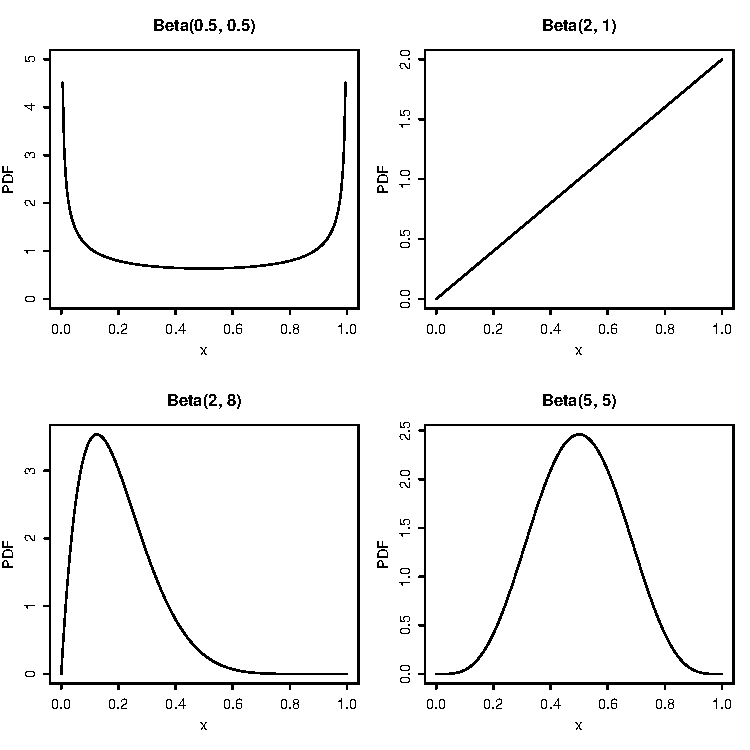
\includegraphics[width=1.9in]{figures/Betapdfs.pdf}
        \end{minipage}
\medskip

\begin{description}

\item[Conjugate Prior of the Binomial] In the Bayesian approach to statistics, parameters are viewed as random variables, to reflect our uncertainty. The \emph{prior} for a parameter is its distribution before observing data. The \emph{posterior}  is the distribution for the parameter after observing data. Beta is the \emph{conjugate} prior of the Binomial because if you have a Beta-distributed prior on $p$ in a Binomial, then the posterior distribution on $p$ given the Binomial data is also Beta-distributed. Consider the following two-level model:
    \begin{align*}
        X|p &\sim \Bin(n, p) \\
        p &\sim \Beta(a, b)
    \end{align*}
Then after observing  $X = x$, we get the posterior distribution
\[p|(X=x) \sim \Beta(a + x, b + n - x) \]

\item[Order statistics of the Uniform] See \emph{Order Statistics}.
\item[Beta-Gamma relationship] If $X \sim \Gam(a, \lambda)$, $Y \sim \Gam(b, \lambda)$, with $X \independent Y$ then
    \begin{itemize}
    	\item $\frac{X}{X + Y} \sim \Beta(a, b)$
    	\item $X + Y \independent \frac{X}{X + Y}$
    \end{itemize}
    This is known as the \textbf{bank--post office result}.
\end{description}


% \[E(X) = \frac{a}{\lambda},  Var(X) = \frac{a}{\lambda^2}\]
% \[X \sim G(a, \lambda),  Y \sim G(b, \lambda),  X \independent Y \rightarrow  X + Y \sim G(a + b, \lambda), \frac{X}{X + Y} \independent X + Y \]
% \[X \sim \Gam(a, \lambda) \rightarrow X = X_1 + X_2 + ... + X_a \textnormal{ for $X_i$ i.i.d. $\Expo(\lambda)$} \]
% \[\Gam(1, \lambda) \sim \Expo(\lambda) \]


\subsection{$\chi^2$ (Chi-Square) Distribution}

Let us say that $X$ is distributed $\chi^2_n$. We know the following:
\begin{description}
    \item[Story] A Chi-Square($n$) is the sum of the squares of $n$ independent standard Normal r.v.s.
    %\item[Example]  The sum of squared errors are distributed $\chi^2_n$
%     \item[PDF] The PDF of a $\chi^2_1$ is:
% \begin{eqnarray*}
% f(w) = \frac{1}{\sqrt{2\pi w}}e^{-w/2},
% w \in [0, \infty)
% \end{eqnarray*}
    \item[Properties and Representations]
\[X \textrm{ is distributed as } Z_1^2 + Z_2^2 + \dots + Z_n^2 \textrm{ for i.i.d.~$Z_i \sim \N(0,1)$}\]
\[X \sim \Gam(n/2,1/2)\]
\end{description}

\section{Discrete Distributions} \smallskip \hrule height 2pt \smallskip

\subsection{Distributions for four sampling schemes}
\begin{center}
    \begin{tabular}{ccc}
        ~ & \textbf{Replace} & \textbf{No Replace}  \\
    \midrule
        \textbf{Fixed \# trials ($n$)} & Binomial & HGeom \\ 
        ~ & (Bern if $n = 1$) & ~ \\ 
        \textbf{Draw until $r$ success} & NBin & NHGeom \\ 
        ~ & (Geom if $r = 1$) & ~\\ \bottomrule
    \end{tabular}
\end{center}

\subsection{Bernoulli Distribution} The Bernoulli distribution is the simplest case of the Binomial distribution, where we only have one trial ($n=1$). Let us say that X is distributed \Bern($p$). We know the following:
\begin{description}
    \item[Story] A trial is performed with probability $p$ of ``success", and $X$ is the indicator of success: $1$ means success, $0$ means failure.
        \item[Example] Let $X$ be the indicator of Heads for a fair coin toss. Then $X \sim \Bern(\frac{1}{2})$. Also, $1-X  \sim \Bern(\frac{1}{2})$ is the indicator of Tails.
        %     \item[PMF.] The probability mass function of a Bernoulli is:
% \[P(X = x) = p^x(1-p)^{1-x}\]
% or simply
% \[P(X = x) = \begin{cases} p, & x = 1 \\ 1-p, & x = 0 \end{cases}\]
\end{description}

\subsection{Binomial Distribution} 
\begin{minipage}{\linewidth}
            \centering
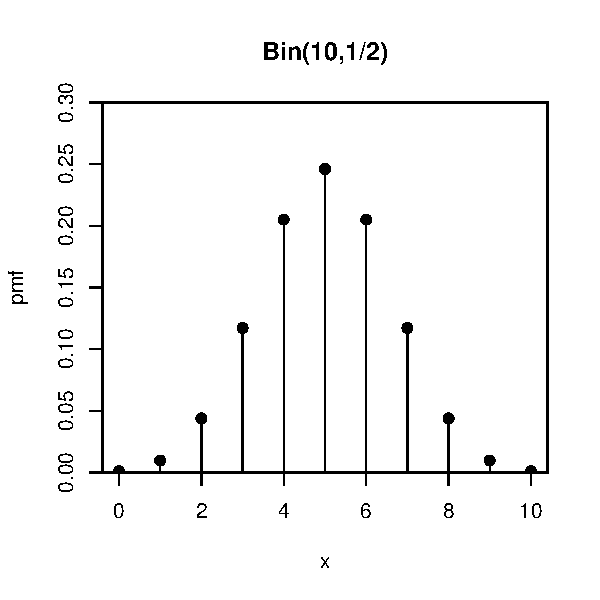
\includegraphics[width=1.3in]{figures/Bin10_05.pdf}
        \end{minipage}

Let us say that $X$ is distributed \Bin($n,p$). We know the following:
\begin{description}
    \item[Story] $X$ is the number of ``successes" that we will achieve in $n$ independent trials, where each trial is either a success or a failure, each with the same probability $p$ of success. We can also write $X$ as a sum of multiple independent $\Bern(p)$ random variables. Let $X \sim \Bin(n, p)$ and $X_j \sim \Bern(p)$, where all of the Bernoullis are independent. Then
        \[X = X_1 + X_2 + X_3 + \dots + X_n\]
    \item[Example] If Jeremy Lin makes 10 free throws and each one independently has a $\frac{3}{4}$ chance of getting in, then the number of free throws he makes is distributed  \Bin($10,\frac{3}{4}$).
    %     \item[PMF] The probability mass function of a Binomial is:
% \[P(X = x) = {n  \choose x} p^x(1-p)^{n-x}\]
\item[Properties] Let $X \sim \Bin(n,p), Y \sim \Bin(m,p)$ with $X \independent Y$.
\begin{itemize}
\item \textbf{Redefine success} $n-X \sim \Bin(n,1-p)$
\item \textbf{Sum} $X+Y \sim \Bin(n+m,p)$
\item \textbf{Conditional} $X|(X+Y=r) \sim \HGeom(n,m,r)$
 \item \textbf{Binomial-Poisson Relationship} $\Bin(n, p)$ is approximately  $\Pois(\lambda)$ if $p$ is small.
   \item \textbf{Binomial-Normal Relationship} $\Bin(n, p)$ is approximately $\N(np,np(1-p))$ if $n$ is large and $p$ is not near $0$ or $1$.
  \end{itemize}
\end{description}

\subsection{Geometric Distribution} Let us say that $X$ is distributed $\Geom(p)$. We know the following:
\begin{description}
    \item[Story] $X$ is the number of ``failures" that we will achieve before we achieve our first success. Our successes have probability $p$.
    \item[Example] If each pokeball we throw has probability  $\frac{1}{10}$ to catch Mew, the number of failed pokeballs will be distributed $\Geom(\frac{1}{10})$.
%     \item[PMF] With $q = 1-p$, the probability mass function of a Geometric is:
% \[P(X = k) = q^kp\]
\end{description}

\subsection{First Success Distribution} Equivalent to the Geometric distribution, except that it includes the first success in the count. This is 1 more than the number of failures. If $X \sim \textnormal{FS}(p)$ then $E(X) = 1/p$.


\subsection{Negative Binomial Distribution} Let us say that $X$ is distributed $\NBin(r, p)$. We know the following:
\begin{description}
    \item[Story] $X$ is the number of ``failures" that we will have before we achieve our $r$th success. Our successes have probability $p$.
    \item[Example] Thundershock has 60\% accuracy and can faint a wild Raticate in 3 hits. The number of misses before Pikachu faints Raticate with Thundershock is distributed $\NBin(3, 0.6)$.
%     \item[PMF] With $q = 1-p$, the probability mass function of a Negative Binomial is:
% \[P(X = n) = {n+r - 1 \choose r -1}p^rq^n\]
\end{description}

\subsection{Hypergeometric Distribution} Let us say that $X$ is distributed $\Hypergeometric(w, b, n)$. We know the following:
\begin{description}
    \item[Story] In a population of $w$ desired objects and  $b$ undesired objects, $X$ is the number of ``successes" we will have in a draw of $n$ objects, without replacement. The draw of $n$ objects is assumed to be a \textbf{simple random sample} (all sets of $n$ objects are equally likely).
    \item[Examples] Here are some HGeom examples.
    \begin{itemize}
    \item Let's say that we have only $b$ Weedles (failure) and $w$ Pikachus (success) in Viridian Forest. We encounter $n$ Pokemon in the forest, and $X$ is the number of Pikachus in our encounters. 
    \item The number of Aces in a 5 card hand.
    \item You have $w$ white balls and $b$ black balls, and you draw $n$ balls. You will draw $X$ white balls.
    \item You have $w$ white balls and $b$ black balls, and you draw $n$ balls without replacement. The number of white balls in your sample is $\HGeom(w,b,n)$; the number of black balls is $\HGeom(b,w,n)$. 
    \item \textbf{Capture-recapture} A forest has $N$ elk, you capture $n$ of them, tag them, and release them. Then you recapture a new sample of size $m$. How many tagged elk are now in the new sample? $\HGeom(n,N-n,m)$
    \end{itemize} 
%    \item[PMF] The probability mass function of a Hypergeometric:
%\[P(X = k) = \frac{{w \choose k}{b \choose n-k}}{{w + b \choose n}}\]
\end{description}

\subsection{Poisson Distribution} Let us say that $X$ is distributed $\Pois(\lambda)$. We know the following:
\begin{description}
    \item[Story] There are rare events (low probability events) that occur many different ways (high possibilities of occurences) at an average rate of $\lambda$ occurrences per unit space or time. The number of events that occur in that unit of space or time is $X$.
    
    \item[Example] A certain busy intersection has an average of 2 accidents per month. Since an accident is a low probability event that can happen many different ways, it is reasonable to model the number of accidents in a month at that intersection as $\Pois(2)$. Then the number of accidents that happen in two months at that intersection is distributed $\Pois(4)$.
    
    \item[Properties]
Let $X \sim \Pois(\lambda_1)$ and $Y \sim \Pois(\lambda_2)$, with $X \independent Y$.

\begin{enumerate}
    \item \textbf{Sum} $X + Y \sim \Pois(\lambda_1 + \lambda_2)$
    \item \textbf{Conditional} $X | (X + Y = n) \sim \Bin\left(n, \frac{\lambda_1}{\lambda_1 + \lambda_2}\right)$
    \item \textbf{Chicken-egg} If there are $Z \sim \Pois(\lambda)$ items and we randomly and independently ``accept" each item with probability $p$, then the number of accepted items $Z_1 \sim \Pois(\lambda p)$, and the number of rejected items $Z_2 \sim \Pois(\lambda (1-p))$, and $Z_1 \independent Z_2$.
\end{enumerate}
    
%     \item[PMF] The PMF of a Poisson is:
% \[P(X = k) = \frac{e^{-\lambda}\lambda^k}{k!}\]
\end{description}


\section{Multivariate Distributions} \smallskip \hrule height 2pt \smallskip


\subsection{Multinomial Distribution}
    Let us say that the vector $\vec{X} = (X_1, X_2, X_3, \dots, X_k) \sim \textnormal{Mult}_k(n, \vec{p})$  where $\vec{p} = (p_1, p_2, \dots, p_k)$.
\begin{description}
    \item[Story]  We have $n$ items, which can fall into any one of the $k$ buckets independently with the probabilities $\vec{p} = (p_1, p_2, \dots, p_k)$.
    \item[Example]  Let us assume that every year, 100 students in the Harry Potter Universe are randomly and independently sorted into one of four houses with equal probability. The number of people in each of the houses is distributed $\Mult_4$(100, $\vec{p}$), where $\vec{p} = (0.25, 0.25, 0.25, 0.25)$.
        Note that $X_1 + X_2 + \dots + X_4 = 100$, and they are dependent.
    \item[Joint PMF]  For $n = n_1 + n_2 + \dots + n_k$,
        \[P(\vec{X} = \vec{n}) =  \frac{n!}{n_1!n_2!\dots n_k!}p_1^{n_1}p_2^{n_2}\dots p_k^{n_k}\]
    \item[Marginal PMF, Lumping, and Conditionals]
    Marginally, $X_i \sim \Bin(n,p_i)$ since we can define ``success" to mean category $i$. If you lump together multiple categories in a Multinomial, then it is still Multinomial. For example, $X_i + X_j \sim \Bin(n, p_i + p_j)$ for $i \neq j$ since we can define ``success" to mean being in category $i$ or $j$. Similarly, if $k=6$ and we lump categories 1-2 and lump categories 3-5, then
        \[ (X_1+X_2,X_3+X_4+X_5,X_6) \sim \Mult_3(n, (p_1+p_2, p_3 + p_4+p_5,p_6))\]
        Conditioning on some $X_j$ also still gives a Multinomial:
        \[X_1, \dots, X_{k-1} | X_k = n_k \sim \Mult_{k-1}\left(n - n_k, \left(\frac{p_1}{1 - p_k}, \dots, \frac{p_{k-1}}{1 - p_k}\right)\right)\]
    \item[Variances and Covariances]  We have  $X_i \sim \Bin(n, p_i)$ marginally, so $\var(X_i) = np_i(1-p_i)$. Also, $\cov(X_i, X_j) = -np_ip_j$ for $i \neq j$.
    \end{description}
    
\subsection{Multivariate Uniform Distribution}
See the univariate Uniform for stories and examples. For the 2D Uniform on some region, probability is proportional to area. Every point in the support has equal density, of value $\frac{1}{\textnormal{area of region}}$. For the 3D Uniform, probability is proportional to volume.

\subsection{Multivariate Normal (MVN) Distribution}
A  vector $\vec{X} = (X_1, X_2, \dots, X_k)$ is  Multivariate Normal if every linear combination is Normally distributed, i.e., $t_1X_1 + t_2X_2 + \dots + t_kX_k$ is Normal for any constants $t_1, t_2, \dots, t_k$. The parameters of the Multivariate Normal are the \textbf{mean vector} $\vec{\mu} = (\mu_1, \mu_2, \dots, \mu_k)$ and the \textbf{covariance matrix} where the $(i, j)$ entry is $\cov(X_i, X_j)$. 

\begin{description}
\item[Properties] The Multivariate Normal has the following properties.
\begin{itemize}
\item Any subvector is also MVN.
\item If any two elements within an MVN are uncorrelated, then they are independent.
\item The joint PDF of a Bivariate Normal $(X,Y)$ with $\N(0,1)$ marginal distributions and correlation $\rho \in (-1,1)$ is 
$$  f_{X,Y}(x,y) = \frac{1}{2 \pi \tau} \exp{\left(-\frac{1}{2 \tau^2} (x^2+y^2-2 \rho xy)\right)},$$
with $\tau = \sqrt{1-\rho^2}.$ 
\end{itemize}
\end{description}

\section{Distribution Properties} \smallskip \hrule height 2pt \smallskip
\subsection{Important CDFs}
\begin{description}
   \item[Standard Normal] $\Phi$
    \item[Exponential($\lambda$)] $F(x) = 1 - e^{-\lambda x}, \textrm{ for } x \in (0, \infty)$
    \item[Uniform(0,1)] $F(x) = x, \textrm{ for } x \in (0, 1)$
\end{description}

\subsection{Convolutions of Random Variables}
A convolution of $n$ random variables is simply their sum. For the following results, let $X$ and $Y$ be \emph{independent}.
\begin{enumerate}
    \item  $X \sim \Pois(\lambda_1)$, $Y \sim \Pois(\lambda_2)$ $\longrightarrow X + Y \sim \Pois(\lambda_1 + \lambda_2)$
    \item  $X \sim \Bin(n_1, p)$, $Y \sim \Bin(n_2, p)$ $\longrightarrow X + Y \sim \Bin(n_1 + n_2, p)$. $\Bin(n,p)$ can be thought of as a sum of i.i.d.~$\Bern(p)$ r.v.s.
    \item  $X \sim \Gam(a_1, \lambda)$, $Y \sim \Gam(a_2, \lambda)$ $\longrightarrow  X + Y \sim\Gam(a_1 + a_2, \lambda)$.  $\Gam(n,\lambda)$ with $n$ an integer can  be thought of as a sum of i.i.d.~Expo($\lambda$) r.v.s.
    \item  $X \sim \NBin(r_1, p)$, $Y \sim \NBin(r_2, p)$ $\longrightarrow  X + Y \sim\NBin(r_1 + r_2, p)$. $\NBin(r,p)$ can  be thought of as a sum of i.i.d.~Geom($p$) r.v.s.
    \item  $X \sim \N(\mu_1, \sigma_1^2)$, $Y \sim \N(\mu_2, \sigma_2^2)$  $\longrightarrow  X + Y \sim \N(\mu_1 + \mu_2, \sigma_1^2 + \sigma_2^2)$
\end{enumerate}

\subsection{Special Cases of Distributions}
\begin{enumerate}
    \item $\Bin(1, p) \sim \Bern(p)$
    \item $\Beta(1, 1) \sim \Unif(0, 1)$
    \item $\Gam(1, \lambda) \sim \Expo(\lambda)$
    \item $\chi^2_n \sim \Gam\left(\frac{n}{2}, \frac{1}{2}\right)$
    \item $\NBin(1, p) \sim \Geom(p)$
\end{enumerate}

\subsection{Inequalities}

\begin{enumerate}
\item \textbf{Cauchy-Schwarz} $|E(XY)| \leq \sqrt{E(X^2)E(Y^2)}$
\item \textbf{Markov} $P(X \geq a) \leq \frac{E|X|}{a}$ for $a>0$
\item \textbf{Chebyshev} $P(|X - \mu| \geq a) \leq \frac{\sigma^2}{a^2}$ for $E(X)=\mu, \var(X) = \sigma^2$
\item \textbf{Jensen} $E(g(X)) \geq g(E(X))$ for $g$ convex; reverse if $g$ is concave
\end{enumerate}


\section{Formulas} \smallskip \hrule height 2pt \smallskip
\subsection{Geometric Series}
\[ 1 + r + r^2 + \dots + r^{n-1} = \sum_{k=0}^{n-1} r^k = \frac{1 - r^n}{1 -r} \]
\[ 1 + r + r^2 + \dots = \frac{1}{1-r} \textnormal{ if $|r|<1$} \]

\subsection{Exponential Function ($e^x$)}
\[ e^x = \sum_{n=0}^\infty \frac{x^n}{n!}= 1 + x + \frac{x^2}{2!} + \frac{x^3}{3!} + \dots = \lim_{n \rightarrow \infty} \left( 1 + \frac{x}{n} \right)^n \]

\subsection{Gamma and Beta Integrals}
You can sometimes solve complicated-looking integrals by pattern-matching to a gamma or beta integral:
\[ \int_0^\infty x^{t-1}e^{-x}\, dx = \Gamma(t) \hspace{1 cm} \int_0^1 x^{a - 1}(1-x)^{b-1}\, dx = \frac{\Gamma(a)\Gamma(b)}{\Gamma(a + b)} \]
Also, $\Gamma(a+1) = a \Gamma(a)$, and $\Gamma(n) = (n - 1)!$ if $n$ is a positive integer. 
\subsection{Euler's Approximation for Harmonic Sums}
\[ 1 + \frac{1}{2} + \frac{1}{3} + \dots + \frac{1}{n} \approx \log n + 0.577 \dots\]
\subsection{Stirling's Approximation for Factorials}
\[ n! \approx \sqrt{2\pi n}\left(\frac{n}{e}\right)^n\]

\section{Miscellaneous Definitions} \smallskip \hrule height 2pt \smallskip

\begin{description}
\item[Medians and Quantiles] Let $X$ have CDF $F$. Then $X$ has median $m$ if $F(m) \geq 0.5$ and $P(X \geq m) \geq 0.5$. For $X$ continuous, $m$ satisfies $F(m)=1/2$. In general, the $a$th quantile of $X$ is $\min \{x: F(x)\geq a\}$; the median is the case $a=1/2$.
\item[log] Statisticians generally use $\log$ to refer to natural log (i.e., base $e$).
\item[i.i.d r.v.s] Independent, identically-distributed random variables.

\end{description}

\section{Distributions in R} \smallskip \hrule height 1pt \smallskip

\bigskip

\begin{center}
\begin{tabular}{cc}
\hline
\textbf{Command} & \textbf{What it does} \\
\hline
\texttt{help(distributions)} & shows documentation on distributions\\
\texttt{dbinom(k,n,p)} & PMF $P(X=k)$ for $X \sim \Bin(n,p)$\\
\texttt{pbinom(x,n,p)} & CDF $P(X \leq x)$ for $X \sim \Bin(n,p)$\\
\texttt{qbinom(a,n,p)} &   $a$th quantile for $X \sim \Bin(n,p)$\\
\texttt{rbinom(r,n,p)} &  vector of $r$ i.i.d.~$\Bin(n,p)$ r.v.s\\
\texttt{dgeom(k,p)} & PMF $P(X=k)$ for $X \sim \Geom(p)$\\
\texttt{dhyper(k,w,b,n)} & PMF $P(X=k)$ for $X \sim \HGeom(w,b,n)$\\
\texttt{dnbinom(k,r,p)} & PMF $P(X=k)$ for $X \sim \NBin(r,p)$\\
\texttt{dpois(k,r)} & PMF $P(X=k)$ for $X \sim \Pois(r)$\\
\texttt{dbeta(x,a,b)} & PDF $f(x)$ for $X \sim \Beta(a,b)$\\
\texttt{dchisq(x,n)} & PDF $f(x)$ for $X \sim \chi^2_n$\\
\texttt{dexp(x,b)} & PDF $f(x)$ for $X \sim \Expo(b)$\\
\texttt{dgamma(x,a,r)} & PDF $f(x)$ for $X \sim \Gam(a,r)$\\
\texttt{dlnorm(x,m,s)} & PDF $f(x)$ for $X \sim \mathcal{LN}(m,s^2)$\\
\texttt{dnorm(x,m,s)} & PDF $f(x)$ for $X \sim \N(m,s^2)$\\
\texttt{dt(x,n)} & PDF $f(x)$ for $X \sim t_n$\\
\texttt{dunif(x,a,b)} & PDF $f(x)$ for $X \sim \Unif(a,b)$\\
\hline
\end{tabular}
\end{center}

The table above gives R commands for working with various named distributions. Commands analogous to \texttt{pbinom}, \texttt{qbinom}, and \texttt{rbinom} work for the other distributions in the table. For example, \texttt{pnorm}, \texttt{qnorm}, and \texttt{rnorm} can be used to get the CDF,  quantiles, and random generation for the Normal.  For the Multinomial, \texttt{dmultinom} can be used for calculating the joint PMF and \texttt{rmultinom} can be used for generating random vectors. For the Multivariate Normal, after installing and loading the \texttt{mvtnorm} package \texttt{dmvnorm} can be used for calculating the joint PDF and \texttt{rmvnorm} can be used for generating random vectors.

%\vspace{4in}


\section{Recommended Resources} \smallskip \hrule height 1pt \smallskip

\bigskip

\begin{itemize}
\item Introduction to Probability Book (\url{http://bit.ly/introprobability})
\item Stat 110 Online (\url{http://stat110.net})
\item Stat 110 Quora Blog (\url{https://stat110.quora.com/})
\item Quora Probability FAQ (\url{http://bit.ly/probabilityfaq})
\item R Studio (\url{https://www.rstudio.com})
\item LaTeX File (\texttt{\href{https://github.com/mynameisjanus/6431xProbability}{github.com/mynameisjanus/6431xProbability}})
\end{itemize}

\begin{center}\emph{Please share this cheatsheet with friends!}\end{center}

\end{multicols*}

\section{Table of Distributions} 

\begin{center}
\renewcommand{\arraystretch}{3.7}
\begin{tabular}{cccccc}
\textbf{Distribution} & \textbf{PMF/PDF and Support} & \textbf{Expected Value}  & \textbf{Variance} & \textbf{MGF}\\
\hline 
\shortstack{Bernoulli \\ \Bern($p$)} & \shortstack{$P(X=1) = p$ \\$ P(X=0) = q=1-p$} & $p$ & $pq$ & $q + pe^t$ \\
\hline
\shortstack{Binomial \\ \Bin($n, p$)} & \shortstack{$P(X=k) = {n \choose k}p^k q^{n-k}$  \\ $k \in \{0, 1, 2, \dots n\}$}& $np$ & $npq$ & $(q + pe^t)^n$ \\
\hline
\shortstack{Geometric \\ \Geom($p$)} & \shortstack{$P(X=k) = q^kp$  \\ $k \in \{$0, 1, 2, \dots $\}$}& $q/p$ & $q/p^2$ & $\frac{p}{1-qe^t}, \, qe^t < 1$\\
\hline
\shortstack{Negative Binomial \\ \NBin($r, p$)} & \shortstack{$P(X=n) = {r + n - 1 \choose r -1}p^rq^n$ \\ $n \in \{$0, 1, 2, \dots $\}$} & $rq/p$ & $rq/p^2$ &  $(\frac{p}{1-qe^t})^r, \, qe^t < 1$\\
\hline
\shortstack{Hypergeometric \\ \Hypergeometric($w, b, n$)} & \shortstack{$P(X=k) = \sfrac{{w \choose k}{b \choose n-k}}{{w + b \choose n}}$ \\ $k \in \{0, 1, 2, \dots,  n\}$} & $\mu = \frac{nw}{b+w}$ &$\left(\frac{w+b-n}{w+b-1} \right) n\frac{\mu}{n}(1 - \frac{\mu}{n})$& messy  \\
\hline
\shortstack{Poisson \\ \Pois($\lambda$)} & \shortstack{$P(X=k) = \frac{e^{-\lambda}\lambda^k}{k!}$ \\ $k \in \{$0, 1, 2, \dots $\}$} & $\lambda$ & $\lambda$ & $e^{\lambda(e^t-1)}$ \\
\hline
\hline
\shortstack{Uniform \\ \Unif($a, b$)} & \shortstack{$ f(x) = \frac{1}{b-a}$ \\$ x \in (a, b) $} & $\frac{a+b}{2}$ & $\frac{(b-a)^2}{12}$ &  $\frac{e^{tb}-e^{ta}}{t(b-a)}$\\
\hline
\shortstack{Normal \\ $\N(\mu, \sigma^2)$} & \shortstack{$f(x) = \frac{1}{\sigma \sqrt{2\pi}} e^{-\sfrac{(x - \mu)^2}{(2 \sigma^2)}}$ \\ $x \in (-\infty, \infty)$} & $\mu$  & $\sigma^2$ & $e^{t\mu + \frac{\sigma^2t^2}{2}}$\\
\hline
\shortstack{Exponential \\ $\Expo(\lambda)$} & \shortstack{$f(x) = \lambda e^{-\lambda x}$\\$ x \in (0, \infty)$} & $\frac{1}{\lambda}$  & $\frac{1}{\lambda^2}$ & $\frac{\lambda}{\lambda - t}, \, t < \lambda$\\
\hline
\shortstack{Gamma \\ $\Gam(a, \lambda)$} & \shortstack{$f(x) = \frac{1}{\Gamma(a)}(\lambda x)^ae^{-\lambda x}\frac{1}{x}$\\$ x \in (0, \infty)$} & $\frac{a}{\lambda}$  & $\frac{a}{\lambda^2}$ & $\left(\frac{\lambda}{\lambda - t}\right)^a, \, t < \lambda$\\
\hline
\shortstack{Beta \\ \Beta($a, b$)} & \shortstack{$f(x) = \frac{\Gamma(a+b)}{\Gamma(a)\Gamma(b)}x^{a-1}(1-x)^{b-1}$\\$x \in (0, 1) $} & $\mu = \frac{a}{a + b}$  & $\frac{\mu(1-\mu)}{(a + b + 1)}$ & messy \\
\hline
\shortstack{Log-Normal \\ $\mathcal{LN}(\mu,\sigma^2)$} & \shortstack{$\frac{1}{x\sigma \sqrt{2\pi}}e^{-(\log x - \mu)^2/(2\sigma^2)}$\\$x \in (0, \infty)$} & $\theta = e^{ \mu + \sigma^2/2}$ & $\theta^2 (e^{\sigma^2} - 1)$ & doesn't exist\\
\hline
\shortstack{Chi-Square \\ $\chi_n^2$} & \shortstack{$\frac{1}{2^{n/2}\Gamma(n/2)}x^{n/2 - 1}e^{-x/2}$\\$x \in (0, \infty) $} & $n$  & $2n$ & $(1 - 2t)^{-n/2}, \, t < 1/2$\\
\hline
\shortstack{Student-$t$ \\ $t_n$} & \shortstack{$\frac{\Gamma((n+1)/2)}{\sqrt{n\pi} \Gamma(n/2)} (1+x^2/n)^{-(n+1)/2}$\\$x \in (-\infty, \infty)$} & $0$ if $n>1$ & $\frac{n}{n-2}$ if $n>2$ & doesn't exist\\
\hline
\end{tabular}
\end{center}


\end{document}
